% Options for packages loaded elsewhere
\PassOptionsToPackage{unicode}{hyperref}
\PassOptionsToPackage{hyphens}{url}
%
\documentclass[
  man]{apa6}
\usepackage{amsmath,amssymb}
\usepackage{iftex}
\ifPDFTeX
  \usepackage[T1]{fontenc}
  \usepackage[utf8]{inputenc}
  \usepackage{textcomp} % provide euro and other symbols
\else % if luatex or xetex
  \usepackage{unicode-math} % this also loads fontspec
  \defaultfontfeatures{Scale=MatchLowercase}
  \defaultfontfeatures[\rmfamily]{Ligatures=TeX,Scale=1}
\fi
\usepackage{lmodern}
\ifPDFTeX\else
  % xetex/luatex font selection
\fi
% Use upquote if available, for straight quotes in verbatim environments
\IfFileExists{upquote.sty}{\usepackage{upquote}}{}
\IfFileExists{microtype.sty}{% use microtype if available
  \usepackage[]{microtype}
  \UseMicrotypeSet[protrusion]{basicmath} % disable protrusion for tt fonts
}{}
\makeatletter
\@ifundefined{KOMAClassName}{% if non-KOMA class
  \IfFileExists{parskip.sty}{%
    \usepackage{parskip}
  }{% else
    \setlength{\parindent}{0pt}
    \setlength{\parskip}{6pt plus 2pt minus 1pt}}
}{% if KOMA class
  \KOMAoptions{parskip=half}}
\makeatother
\usepackage{xcolor}
\usepackage{graphicx}
\makeatletter
\def\maxwidth{\ifdim\Gin@nat@width>\linewidth\linewidth\else\Gin@nat@width\fi}
\def\maxheight{\ifdim\Gin@nat@height>\textheight\textheight\else\Gin@nat@height\fi}
\makeatother
% Scale images if necessary, so that they will not overflow the page
% margins by default, and it is still possible to overwrite the defaults
% using explicit options in \includegraphics[width, height, ...]{}
\setkeys{Gin}{width=\maxwidth,height=\maxheight,keepaspectratio}
% Set default figure placement to htbp
\makeatletter
\def\fps@figure{htbp}
\makeatother
\setlength{\emergencystretch}{3em} % prevent overfull lines
\providecommand{\tightlist}{%
  \setlength{\itemsep}{0pt}\setlength{\parskip}{0pt}}
\setcounter{secnumdepth}{-\maxdimen} % remove section numbering
% Make \paragraph and \subparagraph free-standing
\ifx\paragraph\undefined\else
  \let\oldparagraph\paragraph
  \renewcommand{\paragraph}[1]{\oldparagraph{#1}\mbox{}}
\fi
\ifx\subparagraph\undefined\else
  \let\oldsubparagraph\subparagraph
  \renewcommand{\subparagraph}[1]{\oldsubparagraph{#1}\mbox{}}
\fi
\newlength{\cslhangindent}
\setlength{\cslhangindent}{1.5em}
\newlength{\csllabelwidth}
\setlength{\csllabelwidth}{3em}
\newlength{\cslentryspacingunit} % times entry-spacing
\setlength{\cslentryspacingunit}{\parskip}
\newenvironment{CSLReferences}[2] % #1 hanging-ident, #2 entry spacing
 {% don't indent paragraphs
  \setlength{\parindent}{0pt}
  % turn on hanging indent if param 1 is 1
  \ifodd #1
  \let\oldpar\par
  \def\par{\hangindent=\cslhangindent\oldpar}
  \fi
  % set entry spacing
  \setlength{\parskip}{#2\cslentryspacingunit}
 }%
 {}
\usepackage{calc}
\newcommand{\CSLBlock}[1]{#1\hfill\break}
\newcommand{\CSLLeftMargin}[1]{\parbox[t]{\csllabelwidth}{#1}}
\newcommand{\CSLRightInline}[1]{\parbox[t]{\linewidth - \csllabelwidth}{#1}\break}
\newcommand{\CSLIndent}[1]{\hspace{\cslhangindent}#1}
\ifLuaTeX
\usepackage[bidi=basic]{babel}
\else
\usepackage[bidi=default]{babel}
\fi
\babelprovide[main,import]{english}
% get rid of language-specific shorthands (see #6817):
\let\LanguageShortHands\languageshorthands
\def\languageshorthands#1{}
% Manuscript styling
\usepackage{upgreek}
\captionsetup{font=singlespacing,justification=justified}

% Table formatting
\usepackage{longtable}
\usepackage{lscape}
% \usepackage[counterclockwise]{rotating}   % Landscape page setup for large tables
\usepackage{multirow}		% Table styling
\usepackage{tabularx}		% Control Column width
\usepackage[flushleft]{threeparttable}	% Allows for three part tables with a specified notes section
\usepackage{threeparttablex}            % Lets threeparttable work with longtable

% Create new environments so endfloat can handle them
% \newenvironment{ltable}
%   {\begin{landscape}\centering\begin{threeparttable}}
%   {\end{threeparttable}\end{landscape}}
\newenvironment{lltable}{\begin{landscape}\centering\begin{ThreePartTable}}{\end{ThreePartTable}\end{landscape}}

% Enables adjusting longtable caption width to table width
% Solution found at http://golatex.de/longtable-mit-caption-so-breit-wie-die-tabelle-t15767.html
\makeatletter
\newcommand\LastLTentrywidth{1em}
\newlength\longtablewidth
\setlength{\longtablewidth}{1in}
\newcommand{\getlongtablewidth}{\begingroup \ifcsname LT@\roman{LT@tables}\endcsname \global\longtablewidth=0pt \renewcommand{\LT@entry}[2]{\global\advance\longtablewidth by ##2\relax\gdef\LastLTentrywidth{##2}}\@nameuse{LT@\roman{LT@tables}} \fi \endgroup}

% \setlength{\parindent}{0.5in}
% \setlength{\parskip}{0pt plus 0pt minus 0pt}

% Overwrite redefinition of paragraph and subparagraph by the default LaTeX template
% See https://github.com/crsh/papaja/issues/292
\makeatletter
\renewcommand{\paragraph}{\@startsection{paragraph}{4}{\parindent}%
  {0\baselineskip \@plus 0.2ex \@minus 0.2ex}%
  {-1em}%
  {\normalfont\normalsize\bfseries\itshape\typesectitle}}

\renewcommand{\subparagraph}[1]{\@startsection{subparagraph}{5}{1em}%
  {0\baselineskip \@plus 0.2ex \@minus 0.2ex}%
  {-\z@\relax}%
  {\normalfont\normalsize\itshape\hspace{\parindent}{#1}\textit{\addperi}}{\relax}}
\makeatother

% \usepackage{etoolbox}
\makeatletter
\patchcmd{\HyOrg@maketitle}
  {\section{\normalfont\normalsize\abstractname}}
  {\section*{\normalfont\normalsize\abstractname}}
  {}{\typeout{Failed to patch abstract.}}
\patchcmd{\HyOrg@maketitle}
  {\section{\protect\normalfont{\@title}}}
  {\section*{\protect\normalfont{\@title}}}
  {}{\typeout{Failed to patch title.}}
\makeatother

\usepackage{xpatch}
\makeatletter
\xapptocmd\appendix
  {\xapptocmd\section
    {\addcontentsline{toc}{section}{\appendixname\ifoneappendix\else~\theappendix\fi\\: #1}}
    {}{\InnerPatchFailed}%
  }
{}{\PatchFailed}
\keywords{turn-taking, parent-child interaction, child-directed speech, vocal learning, language development\newline\indent Word count: 5373}
\DeclareDelayedFloatFlavor{ThreePartTable}{table}
\DeclareDelayedFloatFlavor{lltable}{table}
\DeclareDelayedFloatFlavor*{longtable}{table}
\makeatletter
\renewcommand{\efloat@iwrite}[1]{\immediate\expandafter\protected@write\csname efloat@post#1\endcsname{}}
\makeatother
\usepackage{lineno}

\linenumbers
\usepackage{csquotes}
\ifLuaTeX
  \usepackage{selnolig}  % disable illegal ligatures
\fi
\IfFileExists{bookmark.sty}{\usepackage{bookmark}}{\usepackage{hyperref}}
\IfFileExists{xurl.sty}{\usepackage{xurl}}{} % add URL line breaks if available
\urlstyle{same}
\hypersetup{
  pdftitle={A social feedback loop supporting early vocal learning in Tseltal Mayan families},
  pdfauthor={Yuchen Jin1, Juan Méndez Girón2, Gilles Polian2, Kennedy Casey2, \& Marisa Casillas1},
  pdflang={en-EN},
  pdfkeywords={turn-taking, parent-child interaction, child-directed speech, vocal learning, language development},
  hidelinks,
  pdfcreator={LaTeX via pandoc}}

\title{A social feedback loop supporting early vocal learning in Tseltal Mayan families}
\author{Yuchen Jin\textsuperscript{1}, Juan Méndez Girón\textsuperscript{2}, Gilles Polian\textsuperscript{2}, Kennedy Casey\textsuperscript{2}, \& Marisa Casillas\textsuperscript{1}}
\date{}


\shorttitle{Social feedback loop in Tseltal}

\authornote{

The authors made the following contributions. Yuchen Jin: Conceptualization, Formal Analysis, Writing - Original Draft Preparation, Writing - Review \& Editing; Juan Méndez Girón: Data Curation, Resources, Validation; Gilles Polian: Data Curation, Resources, Validation; Kennedy Casey: Data Curation, Project Administration, Writing -- Review \& Editing; Marisa Casillas: Conceptualization, Data Curation, Funding Acquisition, Resources, Project Administration, Supervision, Writing -- Review \& Editing.

Correspondence concerning this article should be addressed to Yuchen Jin, Chicago, IL, USA. E-mail: \href{mailto:yuchenjin@uchicago.edu}{\nolinkurl{yuchenjin@uchicago.edu}}

}

\affiliation{\vspace{0.5cm}\textsuperscript{1} Department of Comparative Human Development, University of Chicago\\\textsuperscript{2} Centro de Investigación y Estudios Superiores en Antropología Social Sureste\\\textsuperscript{3} Department of Psychology, Princeton University}

\abstract{%
How do adult caregivers respond to children's vocalizations in non-child-centric culture, and how is it related to children's language development? The present study examined evidence for the social feedback loop in vocal interaction between adults and children under 2;0 in rural Tseltal Mayan families. We found that Tseltal adults respond more to children's canonical and lexical vocalizations, relative to non-canonical vocalizations, and become increasingly selective for lexicality over age. Such adult responsiveness is linked to a higher likelihood of children producing lexical vocalizations immediately afterwards. Our findings parallel the results in previous US-based studies, underscoring the universal relevance of social feedback loops in adult-child interactions and their significant role in shaping early language development across diverse cultural settings.
}



\begin{document}
\maketitle

\hypertarget{introduction}{%
\section{Introduction}\label{introduction}}

Social, vocal interaction between infants and adults is hypothesized to play an important role in infants' early linguistic development (e.g., Bateson, 1975; Catherine, 1977; Donnelly \& Kidd, 2021; Michael H. Goldstein \& Schwade, 2008; Kuhl, 2007). Vocal and non-vocal turn-taking between infants and caregivers begins as young as two months (Bateson, 1975; Trevarthen \& Aitken, 2001) and, over the course of early childhood, has been associated with linguistic outcomes including more speech-related vocalizations (Ferjan Ramírez, Lytle, \& Kuhl, 2020; Gros-Louis \& Miller, 2018; Gros‐Louis, West, \& King, 2014), more voluble talk (Bergelson et al., 2023), larger vocabulary (Donnelly \& Kidd, 2021; Gros‐Louis et al., 2014; Nguyen, Zimmer, \& Hoehl, 2023) and language-related brain function (Nguyen et al., 2023; Romeo et al., 2018). Prior work on vocal learning links these broader developmental outcomes to moment-to-moment changes in child and adult vocalization during contingent interaction: a social feedback loop. Specifically, caregivers are more likely to respond to infants' advanced vocalizations, which in turn, elicits more advanced subsequent vocalizations from infants. Daylong recordings of US 8- to 48-month-old children's home language environments showed that adults were more likely to respond to speech-related vocalizations compared to other types vocalizations (e.g., cries, laughs, vegetative sounds), and that children are more likely to produce speech-related vocalizations after receiving a contingent adult response to a prior speech-related vocalization (Warlaumont, Richards, Gilkerson, \& Oller, 2014). It is also observed in naturalistic playing between 12-month-old (but not 10-month-old) US infants and their parents that parents' responses to infants' canonical vocalizations are associated with greater subsequent canonical babble production by the infants (Gros-Louis \& Miller, 2018). Experiments manipulating the timing of caregiver responses show that 8- to 10-month-old US infants are more likely to produce canonical babble (i.e., consonant-vowel structured syllables) after receiving contingent responses, compared to non-contingent ones (Michael H. Goldstein, King, \& West, 2003; Michael H. Goldstein \& Schwade, 2008). Taken together, the aforementioned research suggests that social interaction may influence longer-term language development via moment-to-moment interactional behavior: caregivers' selective responses to their children and children's adaptation to their caregivers' response pattern.

However, the aforementioned findings are primarily based on English-speaking US families, and thus reflect encultured modes of caregiver-child interaction that are unlikely to be universal (Gaskins, 2020; Ochs \& Kremer-Sadl, 2020). Caregivers' response pattern is largely a reflection of their beliefs about whether and how much children are capable of reciprocal communication, which suggests a potential for cross-culture variation in early interactions. In the US, particularly in contemporary white and middle-class US communities, caregivers often prioritize and accommodate infants' and young children's interactional bids, with the pedagogical aim of helping them communicate and learn language (Catherine, 1977; Gaskins, 2006; Heath, 1983; Ochs \& Kremer-Sadl, 2020). These culturally-specific beliefs may drive some of the findings we reviewed above: US adult caregivers may frequently engage young children in vocal interaction in a way that accommodates the child's developing linguistic and social abilities and encourages them, in turn, to respond with more desired (i.e., mature) vocalizations. For instance, US adults' responses to children are generally shorter, less complex, and leave longer gaps than their responses to other adults (Steven L. Elmlinger, Schwade, \& Goldstein, 2019). Adults adjust their expectations for how children would vocalize to communicate as they become more proficient language users. Infants' smiles, cries, and sustained gaze elicit maternal vocal response in early infancy but not in later toddlerhood, when maternal vocal responses are reserved more exclusively for children's linguistic vocalizations (Catherine, 1977; Yoo, Bowman, \& Oller, 2018). Recent computational work demonstrates how adults' beliefs about children's skills and intentions influence their interpretations of child vocalizations, shaping the content of adult-child conversation and scaffolding children's early communicative skills (Meylan, Foushee, Wong, Bergelson, \& Levy, 2023). In sum, both the processes of establishing mutual intention and practices around verbal turn-taking are subject to parental beliefs, which are culturally embedded.

In the present work, we examine evidence for a social feedback loop in Tseltal Mayan child-caregiver interaction, where adaptive and contingent vocal behavior cannot be as easily ascribed to caregiver pedagogical aims, as it can be in US-based research.

\hypertarget{early-language-socialization-in-mayan-communities}{%
\subsection{Early language socialization in Mayan communities}\label{early-language-socialization-in-mayan-communities}}

Typical language development in rural Mayan communities proceeds on a similar timeline to that observed in urban Western communities, but with a different set of encultured practices and beliefs around caregivers' role in early child language development (Brown, 2011, 2014; Casillas, Brown, \& Levinson, 2020; Liszkowski, Brown, Callaghan, Takada, \& De Vos, 2012). In their home language environments, Tseltal Mayan infants are directly addressed by adults about as much as US, UK, and Argentinian infants are (Bunce et al., 2020; Casillas et al., 2020; see also De León, 1998). However, ethnographic investigations of Mayan language socialization suggest that adult caregivers may not see directed speech as the most essential for children's early communicative development---rather, children are understood to first develop their communicative and linguistic skills as side participants in adult-centered interaction (Brown, 1998; De León, 1998, 2011; Pye, 2022; Vogt, 1969). For most of their first year, infants are carried by a caregiver most of the time during the day, giving them close and frequent access to their caregiver's interactions with others. During this early period of infancy, caregivers' responses to infants' (non-linguistic) vocalizations, gestures, and actions focus a great deal on simple social routines, and caregivers may quote infants' apparent intentional communicative behaviors as a kind of proto-speech (De León, 1998). When infants become more mobile, around 10 months of age, caregivers begin to address them more often with utterances to manage their behavior. Then, later, the onset of clear dyadic conversation is observed to be initiated by developmental changes of the child rather than the caregiver---when children start to produce one-word utterances, caregivers respond (De León, 1998). Thus, Mayan children's ability to produce words may be crucial for achieving adults' recognition of them as potential interlocutors. In sum, Mayan children are brought into the adult social world first as side participants before gaining rights as ratified interlocutors---a status achieved once they become recognizable as competent language producers (Brown, 2011, 2014; De León, 2011).

Among all of these reviewed findings, two important pieces of evidence stand out in furthering our hypothesis: (1) research on US communicative development finds that non-word canonical babble sequences are key in the realization of an early social feedback loop for vocal learning, while (2) research on Mayan language socialization suggests that infants' first lexical utterances are key for the initiation of dyadic interaction---in which a similar feedback loop would presumably emerge. In this case, we expect that social feedback loops vary cross-culturally in their basic requirements and behaviors, which may bring up different impacts on language development. That said, given the limited work on Mayan child-caregiver vocal interaction before age 1;6, we can't rule out the possibility that social feedback loops for early vocal behavior are driven by similar mechanisms---even across groups with ideologically distinct approaches to infant communication---but we simply haven't yet observed enough data. In reality, these two outcomes are not mutually exclusive (e.g., ideology may shape the content of a response more than the provision of a response), but we here draw the two possibilities as distinct to illustrate the extent to which one might expect cross-cultural similarity or difference to emerge in early child-caregiver interaction. Based on prior work, we might predict that a social feedback loop for vocal behavior in Mayan interactions becomes clear only later, when children begin to produce words---not earlier, when they begin to produce canonical (non-word) babble.

\hypertarget{the-present-study}{%
\subsection{The present study}\label{the-present-study}}

In the present study, we asked two questions about Tseltal Mayan child-caregiver interaction under age two (0;2--2;0):

\begin{enumerate}
\def\labelenumi{\arabic{enumi}.}
\item
  What linguistic features of children's early speech drive adults to respond (speech-like babble, words, or both)? Based on prior work, we predicted that responsiveness would be driven by children's use of intelligible words rather than children's speech-like non-word babble (Brown, 2011, 2014; De León, 1998, 2011).
\item
  Does adults' responsiveness predict an increased use of these linguistic features in children's subsequent vocal production? Based on the robustness of social feedback effects in the prior literature, we predicted that adult responses to language-like vocalizations would be associated with a greater likelihood of children continuing to produce language-like vocalizations.
\end{enumerate}

We examined these predictions while controlling for both child age (older children produce more linguistically sophisticated utterances; affecting predictions 1 and 2), current interlocutor engagement (responsiveness is higher within vs.~outside of interactional bursts; affecting prediction 1), and the infants' immediately prior vocalization (infant lexical vocalizations are more likely following prior infant lexical vocalizations; affecting prediction 2).

\hypertarget{method}{%
\section{Method}\label{method}}

\hypertarget{corpus}{%
\subsection{Corpus}\label{corpus}}

The audio recordings on which the present data were based were collected by the final author in 2015--2018 in a rural farming community located in the municipality of Tenejapa, Chiapas, Mexico (Casillas et al., 2017). During the day, 55 children under age five wore a vest containing a lightweight stereo audio recorder (Olympus WS-832, Olympus Corporation, Tokyo, Japan) to capture the child's vocalizations and their surrounding linguistic environment. The recordings were usually 9 to 11 hours long and took place in and around children's homes when the researcher was not present.

We randomly sampled 9 five-minute clips from daylong audio recordings of 32 Tseltal children (16 female) age 2;0 and younger (median=7.50, range=2--24). Only fully annotated clips (see Annotation section for detailed descriptions) were included in the current study (median=6/child, range=1--8/child), each of which contained at least one case of child vocalization. Most children lived with more than two caregivers, and the average household size was 6 people. Most (84\%) mothers and all fathers had some school experience: 31\% of mothers and 50\% of fathers had completed secondary or higher levels of education. Two children were reported to be learning both Tseltal and Spanish in the home, while the other thirty were only reported to be learning Tseltal. That said, all children were likely exposed to some amount of Spanish via lexical borrowings into Tseltal, Spanish-based television and radio, and nearby adult conversations involving non-Tseltal community members or Tseltal-Spanish bilinguals who prefer to express themselves in both languages.

These clips were then annotated for all target-child-produced and target-child-directed linguistic vocalizations. That is, any instance of words and babble (i.e., not cries, laughs, or vegetative sounds) that were either produced by the target child or directly addressed to the target child, were transcribed in Tseltal and loosely translated into Spanish. All transcription and loose translation was completed in ELAN (Sloetjes \& Wittenburg, 2008) by the second author, who is a native Tenejapan Tseltal speaker.

\hypertarget{annotation}{%
\subsection{Annotation}\label{annotation}}

On a first pass through the transcribed data, we first checked and, if necessary, edited the onset and offset boundaries of each utterance to ensure that the timing was precise with respect to the acoustic signal. In this process of comprehensive transcript review, several other corrections in diarization arose, including: potential missed target child speech, over-attribution of target child speech (other children's speech or non-linguistic target child vocalizations), and the inclusion of other-child-directed speech. These potential corrections were proposed by authors YC, KC, and three research assistants they managed---each trained in the ACLEW Annotation Scheme (Casillas et al., 2017). Potential corrections were sent back to author XMG, a native Tenejapan Tseltal speaker, who confirmed or rejected them as necessary. Each transcript passed through this loop of review until there were no further proposed corrections.

The final transcripts included annotations indicating (1) whether each vocalization was a contingent response to a prior vocalization (yes/no), (2) whether each vocalization took place within an interactional burst (yes/no), and (3) the vocal maturity status of target children's vocalizations (lexical \textgreater{} canonical but non-lexical \textgreater{} neither canonical nor lexical). We describe each of these three annotation types in turn.

A child's utterance was counted as receiving a contingent response if an adult produced target-child-directed speech within 2 seconds of the child's utterance offset. For children of this age and with this type of naturalistic recording, we can expect most child-adult conversational turn transitions to occur within 2 seconds (Casillas, Bobb, \& Clark, 2016; Casillas \& Scaff, 2021; Hilbrink, Gattis, \& Levinson, 2015; Nguyen et al., 2023). Prior work has also used this 2-second cutoff to classify responses as contingent or non-contingent (e.g., Steven L. Elmlinger, Goldstein, \& Casillas, 2023; Michael H. Goldstein \& Schwade, 2008), allowing us to make stronger links to prior findings on the social feedback loop. This annotation was conducted in RStudio (R Core Team, 2020) based on the boundaries of utterances.

A child's utterance was coded as within an ongoing interactional burst if it followed an adult's target-child-directed utterance within 2 seconds. We annotated whether the vocalization occurred within an interactional burst because it serves as an indicator of the adult interlocutor's attention---we expect a response to the child's vocalization to be more likely if the adult has recently been responding to the child, than if the child vocalizes during a period of interactional silence. Bursty distributions of linguistic input are themselves a topic of theoretical interest (Abney, Dale, Louwerse, \& Kello, 2018; Casillas et al., 2020; Goh \& Barabási, 2008; Slone, Abney, Smith, \& Yu, 2023; Catherine S. Tamis-LeMonda, Kuchirko, Luo, Escobar, \& Bornstein, 2017), while here we consider it as a control factor in trying to understand patterns of adult responsiveness. This annotation was also conducted in RStudio (R Core Team, 2020) based on the boundaries of utterances.

Vocal maturity annotations were completed manually by classifying each vocalization into one of three types: non-canonical and non-lexical, canonical but non-lexical, or lexical. Canonical vocalizations must (a) contain both consonant and vowel elements and (b) feature speech-like (smooth and rapid; \textless120 ms) transition timing between the consonant- and vowel-like portions of the syllable. Utterances with a mix of canonical and non-canonical syllables were labeled as canonical. An utterance was marked as lexical, if it contained at least one recognizable word. Expressives such as ``oh'' and ``ah'' were counted as a word, if they were meant to be communicative, based on the judgment of the native Tseltal-speaking author. Lexical utterances were counted as such regardless of whether they were canonical or not. Both lexical utterances and canonical utterances were regarded as language-like vocalizations, and non-lexical, non-canonical utterances were non-language-like vocalizations. In our vocal maturity ranking, lexical utterances were the most mature and non-lexical, non-canonical utterances were the least. Thirty transcripts containing at least one child-produced utterance were randomly selected to be double coded during the first coding pass. Annotators agreed on 81.32\% of non-canonical versus canonical classifications and 89.11\% of non-lexical versus lexical classifications. Following the final transcript corrections by XMG, a native Tenejapan Tseltal speaker, all vocal maturity annotations were checked and corrected as needed by KC.

\hypertarget{results}{%
\section{Results}\label{results}}

All analyses and plots were conducted in RStudio (R Core Team, 2020) using the tidyverse (Wickham et al., 2019) and lme4 (Bates, Mächler, Bolker, \& Walker, 2015) packages. A reproducible manuscript in which these analyses can be inspected on the basis of anonymized data are publicly available at the following repository: \url{https://github.com/Regenchen/Tseltal-turn-taking/tree/145847cef20ab3f79242c52459eaf57fa5b4db71/data}.

\hypertarget{tseltal-childrens-vocal-development}{%
\subsection{Tseltal children's vocal development}\label{tseltal-childrens-vocal-development}}

We first verified whether the vocal maturity data in our new corpus align with expectations based on the literature at large, as well as prior work on vocal maturity in this community (Casillas et al., 2020). Overall, we found that the 32 children produced, on average, 5.28 vocalizations/minute (median=4, range=0.20--24). As shown in Figure~\ref{fig:vcm-trajectories-plot}, children begin by exclusively producing non-canonical and non-lexical vocalizations. Then, between 0;6 and 1;0, there is a decline in the use of non-canonical babble and an increase in the use of canonical babble. Recognizable words are observed as early as 0;6, picking up speed just before 1;0 and continuing to increase across the rest of the observed age range \footnote{This effect still came out when age was treated as a continuous variable.}. This trajectory aligns with previous research on Tseltal children's language development and is also quite similar to what we know about US children.

\begin{figure}
\centering
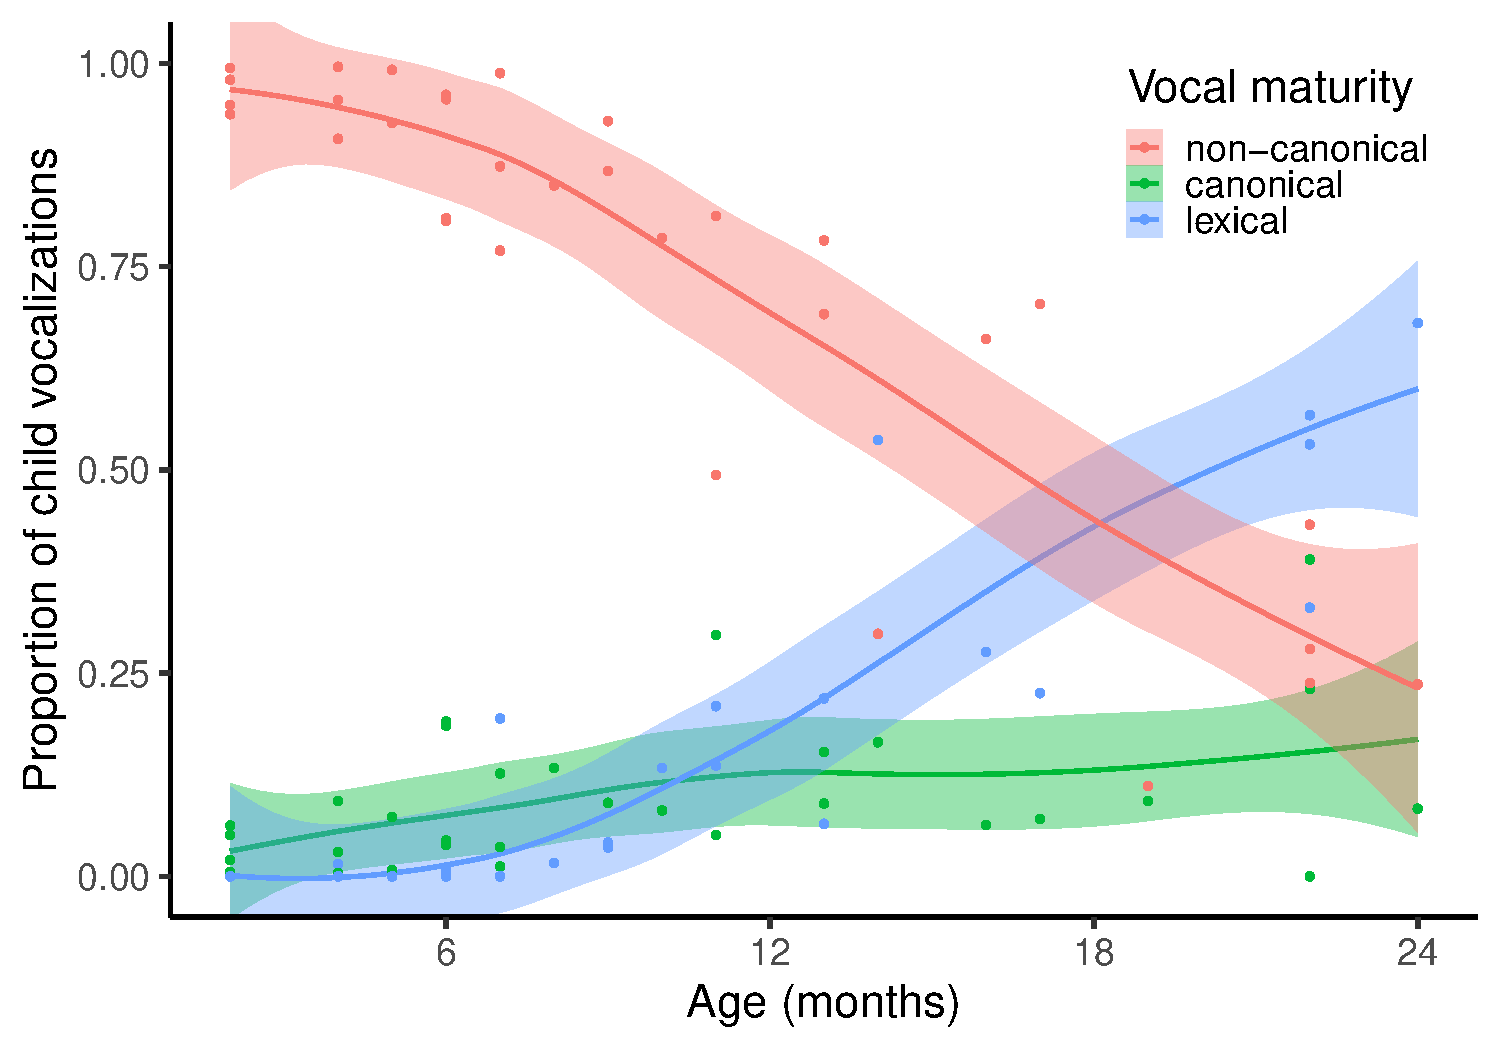
\includegraphics{turntaking_paper_files/figure-latex/vcm-trajectories-plot-1.pdf}
\caption{\label{fig:vcm-trajectories-plot}The proportions of child vocalizations that are non-canonical (red dots and curve), canonical (green dots and curve), and lexical (blue dots and curve) at different ages between 2 and 24 months. The curves are based on local regression.}
\end{figure}

\hypertarget{overall-target-child-directed-input}{%
\subsection{Overall target child-directed input}\label{overall-target-child-directed-input}}

Overall, the 32 target children heard 14 target-child-directed utterances, coming to a rate of 1.77 vocalizations per minute (median=1.40, range=0.20--8.60), among which 66.63\% from women, 21.37\% from girls, 7.53\% from men, and 4.46\% from boys. That is, these children received more directed input from female speakers compared to male speakers, and more from adults compared to other children. Adult caregivers produced 1.44 child-directed utterances/minute (median=0.80, range=0.20--8.60). Of the 1,329 child-directed utterances produced by adults, only 10\% of target children's utterances received a temporally contingent adult response (i.e., appearing within two seconds of offset of the preceding child utterance), which is lower than a previous estimate of \textasciitilde20\% observed with a smaller and broader age ranging sample of Tseltal children (N=10, age range=0;2-3;0, (Steven L. Elmlinger et al., 2023)).

\hypertarget{adults-responsiveness-according-to-childrens-interlocutor-features}{%
\subsection{Adults' responsiveness according to children's interlocutor features}\label{adults-responsiveness-according-to-childrens-interlocutor-features}}

We used logistic mixed-effects regression \footnote{This effect still came out when age was treated as a continuous variable.} to predict whether a child's utterance received a response (yes/no), given the utterance's vocal maturity (non-canonical/canonical/lexical), the target child's age in months (scaled), and their two-way interaction. To this base model, we added whether the utterance occurred within an interactional burst (yes/no) and a two-way interaction between interaction burst status and age. As described above, we expected that target child vocalizations produced within an ongoing interaction would have a higher overall likelihood of receiving a response. This pattern may be sensitive to child age; compared to older children, younger children who are more often treated as side participants are less likely to succeed in eliciting adults' response when they are not situated in ongoing interactions. Finally, we added by-child random intercepts.

More vocally mature utterances were significantly more likely to receive a temporally contingent adult response (Figure~\ref{fig:adult-response-model-plot}). Adults were more likely to respond to target children's canonical (\(\beta\) = 0.55, \emph{SE} = 0.18, \emph{z} = 3.09, \emph{p} = 0.00) and lexical vocalizations (\(\beta\) = 0.64, \emph{SE} = 0.19, \emph{z} = 3.29, \emph{p} = 0.00), compared to non-canonical (and non-lexical) vocalizations. We found no evidence for differences in adults' response rate to target children's canonical versus lexical vocalizations. A significant interaction effect of age and vocal maturity (\(\beta\) = 0.48, \emph{SE} = 0.18, \emph{z} = 2.67, \emph{p} = 0.01) revealed that the difference between adults' temporal responsiveness to children's lexical versus non-canonical vocalizations was larger for older children. And, while adult responses were indeed more likely when target children vocalized within an ongoing interactional burst (\(\beta\) = 1.90, \emph{SE} = 0.13, \emph{z} = 14.21, \emph{p} = 0), the effects of vocal maturity and age were apparent for both within-burst and outside-of-burst target child vocalizations (Figure~\ref{fig:adult-response-model-plot}).

\hypertarget{childrens-vocal-production-following-adults-responses}{%
\subsection{Children's vocal production following adults' responses}\label{childrens-vocal-production-following-adults-responses}}

We used logistic mixed-effects regression \footnote{This effect still came out when age was treated as a continuous variable.} to predict whether a child's utterance was lexical (yes/no), given whether the child's immediately prior utterance was responded to by an adult (yes/no), the target child's age in months (6--12mo/12--18mo/18--24mo) \footnote{This effect still came out when age was treated as a continuous variable.}, and their two-way interaction. Because children younger than 6 months old did not produce lexical speech, we only included data for children older than 6 months of age (\emph{N}=19). We classified children's age into three bins because children's lexical production experiences a non-linear surge at around 18 months of age. As a control variable, we then added whether the child's immediately prior utterance was also lexical; as described above, we expected lexical child vocalizations to be more likely following prior lexical child vocalizations. Finally, we also included by-child random intercepts.

As results showed, children were significantly more likely to produce lexical vocalizations when their immediately prior vocalization was responded to contingently by an adult (\(\beta\) = 1.01, \emph{SE} = 0.34, \emph{z} = 2.92, \emph{p} = 0.00). While as expected, lexical vocalizations are more likely to follow prior lexical vocalizations, and to appear in 18- to 24-month-old children' speech than 6-12 months (but not 12-18 months), the effect of adult response is significant for all three age groups, regardless of whether prior vocalization is lexical or not (Figure~\ref{fig:social-loop-plot}).

\begin{figure}
\centering
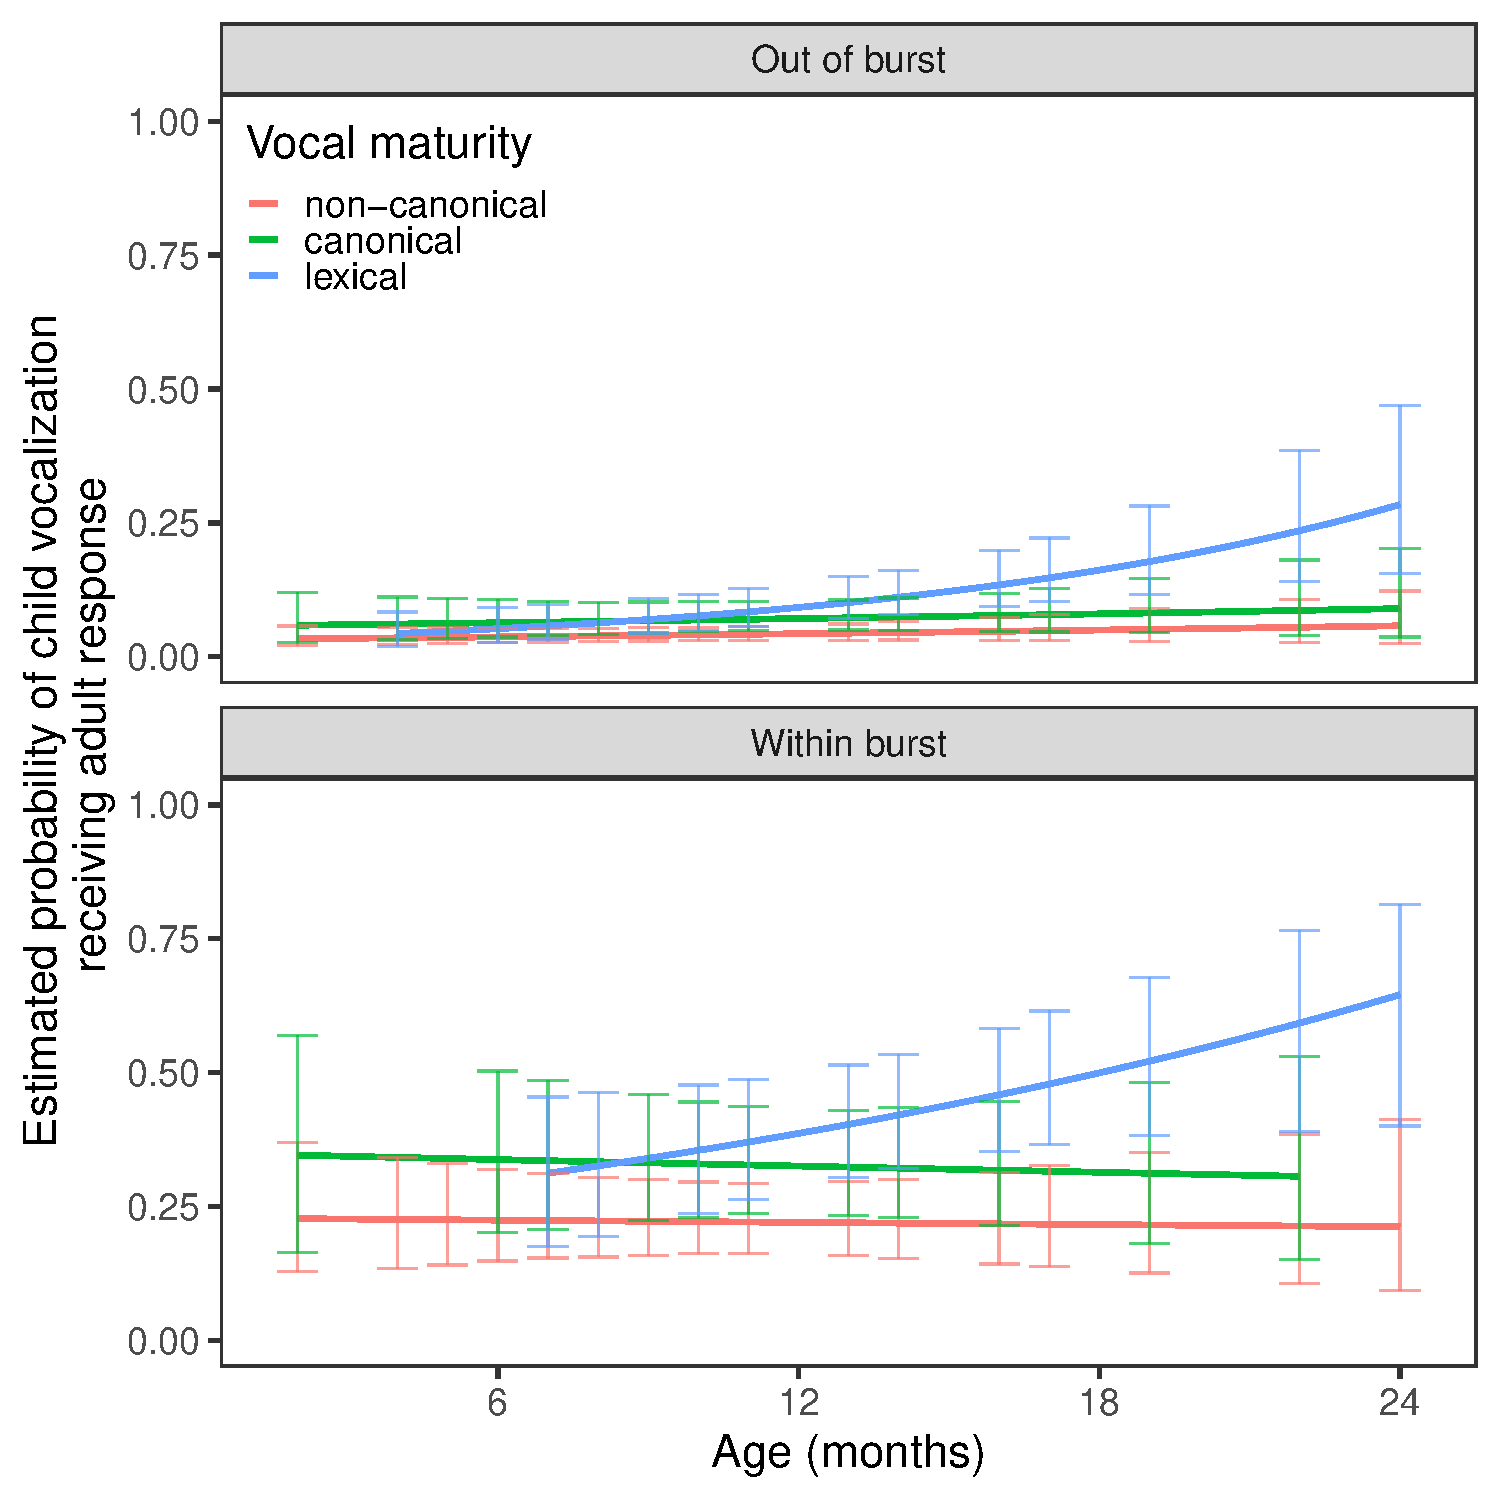
\includegraphics{turntaking_paper_files/figure-latex/adult-response-model-plot-1.pdf}
\caption{\label{fig:adult-response-model-plot}The estimated probability of children's non-canonical (red), canonical (green), and lexical (blue) vocalizations that receive adult response at different ages between 2 and 24 months, either out of conversation burst (left facet) or within burst (right facet). Error bars indicate the variability or confidence interval for each point estimate.}
\end{figure}

\begin{figure}
\centering
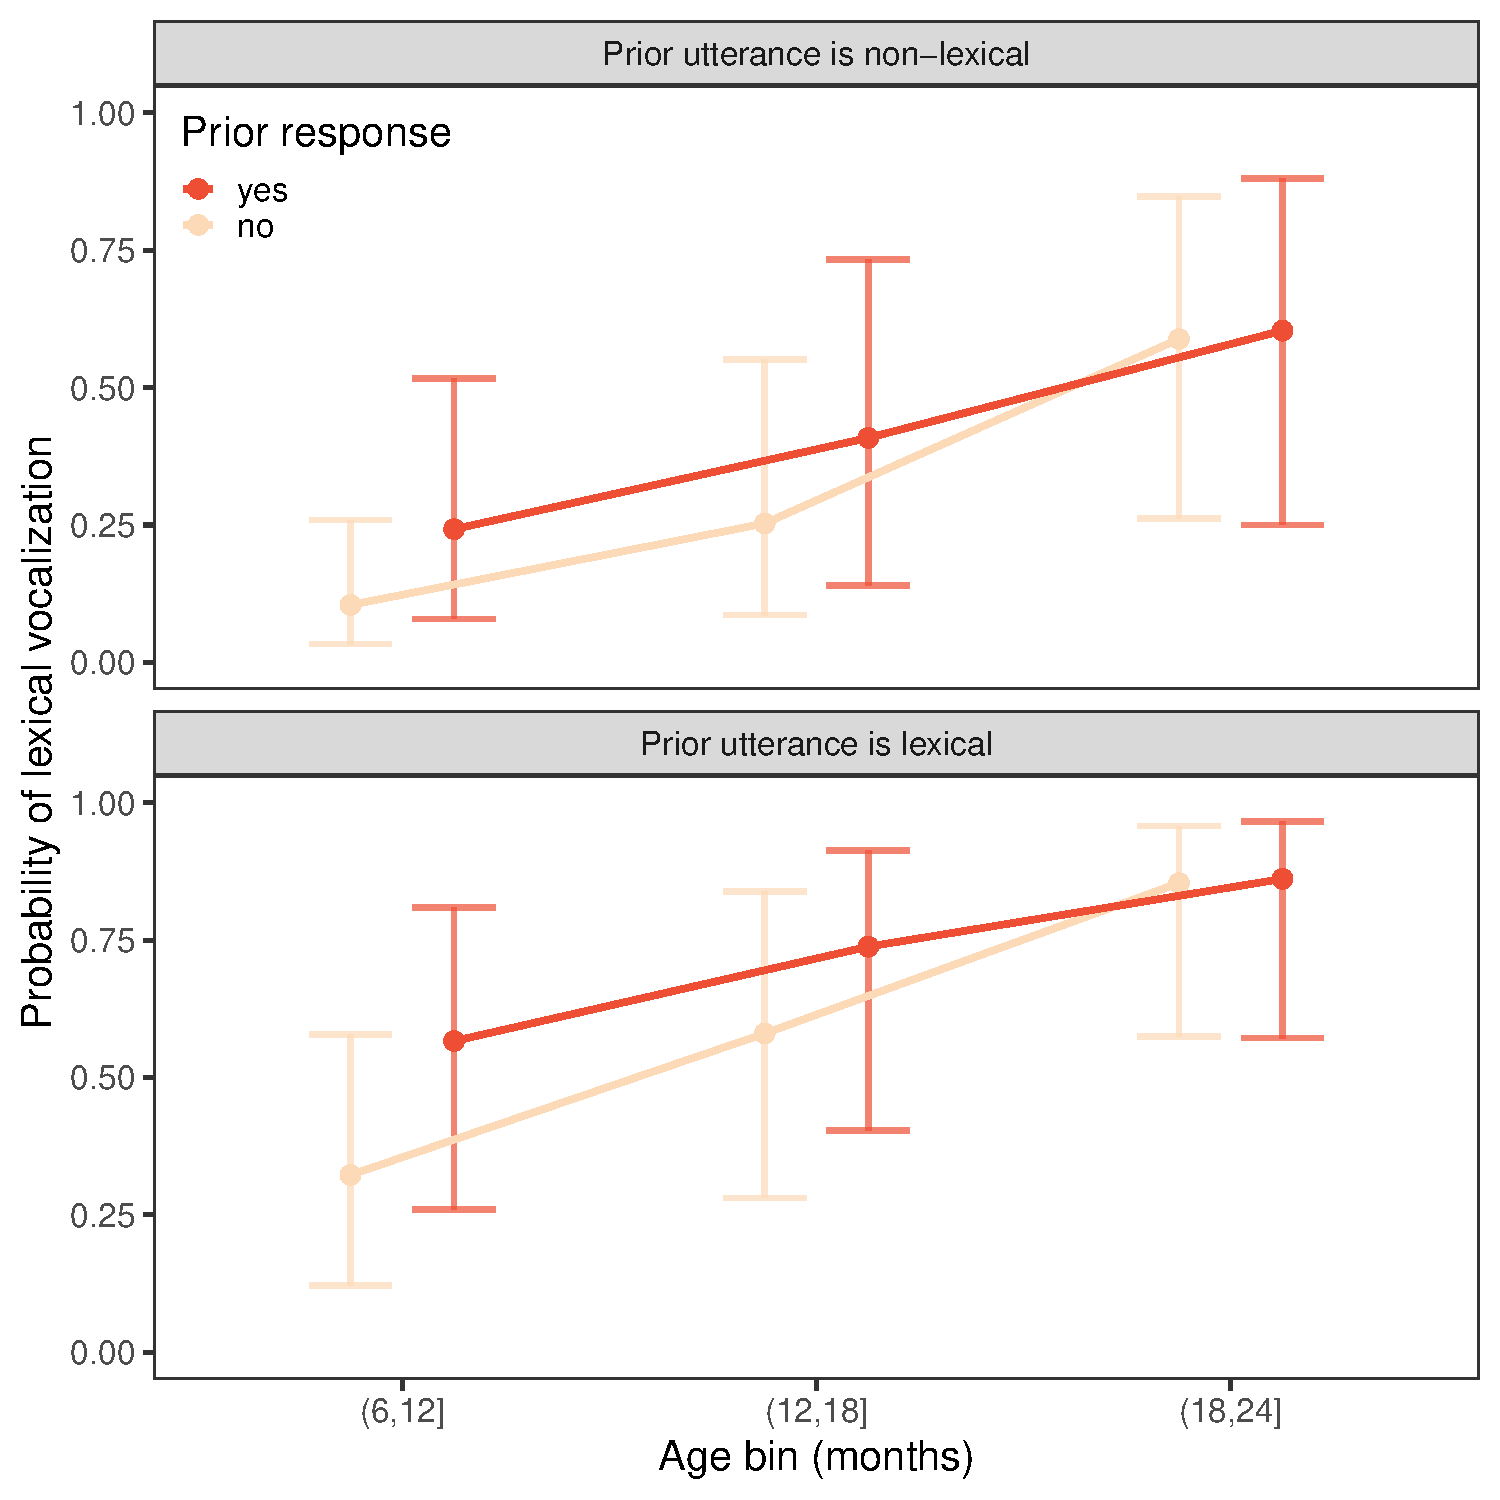
\includegraphics{turntaking_paper_files/figure-latex/social-loop-plot-1.pdf}
\caption{\label{fig:social-loop-plot}The estimated probability of children's vocalizations that are lexical at 6 to 12 months old, 12 to 18 months old and 18 to 24 months old, given their prior utterance is responded to by an adult (red) or not (light orange), and whether their prior utterance is non-lexical (left facet) or lexical (right facet). Error bars indicate the variability or confidence interval for each point estimate.}
\end{figure}

\hypertarget{discussion}{%
\section{Discussion}\label{discussion}}

The present study examined evidence for a social feedback loop in the vocal learning of Tseltal-acquiring infants. Social feedback loops provide a moment-to-moment mechanism for the longer-term influence of social interactions on linguistic and communicative development. Prior work on these feedback loops for vocal learning highlights canonical (speech-like) babble as an inflection point in the development of these loops---canonical babble elicits adult responses that encourage further canonical babble. However, past work on these loops for vocal learning has come almost exclusively from urban and suburban US English-speaking populations, in which these interactive accommodations by adults can be understood as US caregivers' intentional, belief-driven efforts to engage children in conversations and facilitate their communicative and linguistic skills. To better understand how social feedback loops function in different cultural contexts, the present study examined vocal interaction between adults and children under 2;0 in rural Tseltal Mayan families, where ethnographic evidence led us to predict that feedback loops in vocal behavior would be driven by and elicit recognizable lexical utterances, more so than (non-lexical) canonical babble.

Different from our expectations, we found no evidence that lexical vocalizations play a unique role in Tseltal vocal feedback loops; mirroring prior US data, both lexical utterances and non-lexical canonical babble heightened the chance of a contingent adult response, with no significant difference between response rates to these two more vocally mature categories. In other words, the Tseltal caregivers' responsiveness patterned similarly to US caregivers' documented in prior work (Michael H. Goldstein et al., 2003; Michael H. Goldstein \& Schwade, 2008; Miller \& Gros-Louis, 2013).

Otherwise the results generally patterned as expected: adults were more exclusively responsive to lexical vocalization for older children, adult response was more likely when a child's vocalization occurred within an ongoing interactional burst. Children were more likely to produce a lexical vocalization when their immediately prior vocalization was responded to by an adult or was, itself, lexical. Finally, older children were more likely to produce more vocally mature vocalizations.

These findings add to our descriptive basis of vocal development in Tseltal and suggest that social feedback loops are a salient pattern of adult-child interaction across different caregiving approaches and cultural contexts.

\hypertarget{becoming-a-tseltal-interactant}{%
\subsection{Becoming a Tseltal interactant}\label{becoming-a-tseltal-interactant}}

In these data, Tseltal adults began the process of drawing children in as interlocutors somewhat earlier than previously observed---in response to canonical babble, which emerges earlier than lexical speech (Brown, 2014; Casillas et al., 2020). Although Tseltal adults may see children's communicative and linguistic competence as developing first through side participation (i.e., indirectly addressed language) until children produce their first recognizable words (De León, 1998, 2011), early social feedback loops for vocal behavior begin even earlier: when children start to produce canonical babble. Adult caregivers also adjusted their response patterns across early linguistic development, demonstrating sensitivity to their interlocutor that has been observed with infant-caregiver interactions in other cultural contexts {[}e.g., English families; Catherine (1977){]}. These patterns in moment-to-moment adaptation may then derive from heuristics for coordination that apply much more broadly beyond the adult-infant interactions (e.g., adult interactions: Clark, 1996; Levinson, 2006; non-human animals: Michael H. Goldstein et al., 2003).

Nevertheless, cultural differences may materialize in other dimensions of interaction and early turn taking that were not explored in the current study, such as the content of the adult responses. For instance, behavioral management utterances (De León, 1998) and dialogic repetitions (Brown, 1998) are salient in Tseltal adults' child-directed speech, but may be less frequently observed in many US contexts (Newport, Gleitman, \& Gleitman, 1977). Tseltal infants are exposed many times a day to adults' greeting routines during coming and going but are typically not themselves directly greeted (De León, 1998; Foushee \& Srinivasan, 2023), meanwhile, routine words such as hi and bye-bye are frequent in child-directed speech for US English-learning children (e.g., Casey, Potter, Lew-Williams, \& Wojcik, 2023). We suspect that an examination of the content of these utterances would produce an analysis that reflects a Tseltal- and Mayan-specific approach to language socialization.

The findings also shed light on how Tseltal children glean linguistic knowledge from their interactions with adults. While rural Tseltal infants are directly addressed by adults about as much as infants in US, UK, and Argentinian urban families (Bunce et al., 2020; Casillas et al., 2020), ethnographic report suggests that adult Mayan caregivers instead see children's side participation in adult interaction as the key arena for pre-verbal communicative and linguistic development (Brown, 1998; De León, 1998, 2011; Pye, 2022; Vogt, 1969). The current study shows that, even during the pre-verbal period, adult caregivers are occasionally making contingent responses to child vocalizations, and that their responses are increasingly selective for age-appropriate vocally mature utterances across the first two years. Children picked up on this invitation, yielding further mature vocalizations, and ultimately a route to verbal turn-taking.

Meanwhile, we cannot ignore the potential contribution of the large amount of other-directed speech overhearable to children---which occurs at a rate of 5--6 times that of directed speech in this community (Casillas et al., 2020). Especially considering that Tseltal children are socialized as side participants from an early age (Clark, 1996; De León, 1998; Foushee \& Srinivasan, 2023), adults' responsiveness to infant vocalizations is only one of many resources from which Tseltal children pick up and practice communicative and linguistic skills.

\hypertarget{early-turn-taking-behaviors-across-cultures}{%
\subsection{Early turn-taking behaviors across cultures}\label{early-turn-taking-behaviors-across-cultures}}

Even though parenting ideologies and language socialization practices vary across cultures, we can still observe some patterns that are comparable and salient, perhaps the outcome of basic principles of coordination and conversational interaction that are tailored and adapted by linguistic communities around the world (Clark, 1996; Levinson, 2006) ---these ``basic principles'' theories are primarily evolutionary in nature, and put the infant-caregiver interactions we observe here in a much more expansive context. For example, we can interpret our current findings in the framework of joint action, under a circumstance where there can be little common ground assumed beyond shared percepts between a preverbal infant and their adult caregiver (Clark, 1996) ---if the adult sees it possible to bring the child into a conversation-like format, they might try and coax this joint action from the infant through selective contingent response for conversation-like structure (turn taking) and language-like vocalization (canonical babble and/or lexical speech). Michael H. Goldstein et al. (2003) see this behavior through a multi-species lens, in which the provision and adaptation of contingent response by mature organisms to immature ones is a generalized and instinctually rooted mechanism for the transmission of animal communication systems. The Human Interaction Engine Hypothesis (Levinson, 2006) would see things somewhat differently, highlighting instead the human-specific aspects of these early instincts for turn-taking structure as building an framework for dynamic, multimodal, and intersubjective engagement between infant and caregiver, in which language development is adapted to unfold.

In each of these cases, the theoretical puzzle is to link children's experiences with language to their linguistic development. While social feedback has been linked to language learning across multiple aspects of linguistic development (Kuhl, 2007; Rowe \& Snow, 2020; Catherine S. Tamis-LeMonda, Kuchirko, \& Song, 2014), the mechanism that our current findings touch upon is more likely to operate over the timescale of seconds or minutes, which could be underpinned by basic biological or neural processes for behavioral entrainment and synchrony (Nguyen et al., 2021; Wass, Whitehorn, Marriott Haresign, Phillips, \& Leong, 2020).

That said, we do not wish to imply equivalent roles of social feedback loops for language learning across culturally diverse communities. The existence of similar interactional structures for language sheds light on shared mechanisms for language learning and processing but does not imply total parallelism. Rather, based on prior literature and current theory, we can expect substantial room for cross-linguistic and cross-cultural variation in how children learn the grammar, words, and practices for using their home language(s). For example, as mentioned, the vast majority of Tseltal children's linguistic input comes through overhearing rather than in direct speech. While our findings suggested the social feedback loop between adults and infants exists in Tseltal families as it does in US families, the same phenomena may carry different weight for communicative and linguistic development in different cultural contexts.

\hypertarget{limitations-and-future-research}{%
\subsection{Limitations and future research}\label{limitations-and-future-research}}

We used turn transition timing as the criteria for selecting contingent turns, yet it is possible for two unrelated utterances to be temporally contingent (child: ``want more'' --- caregiver: ``oh, say hi to brother''). More detailed annotation is needed to address this issue. That said, temporal contingency itself can make an utterance salient to the interlocutor, particularly for young children who haven't acquired adult-like lexical and pragmatic knowledge.

Future research may want to dig deeper into how social feedback works to support early vocal learning. One possibility is that any contingent adult response---even non-verbal responses---serves as a positive reinforcement of children's language-like vocalizations. So, non-verbal responses such as laughing, soothing, and action (e.g., giving an object, feeding) can also facilitate early vocal development. Another possible mechanism is that conversational turn-taking encourages infants to incorporate phonetic features of adult speech, which contributes to successful communication and ultimately pushes children toward linguistically mature conversationalists. Research with adults shows that when they are asked to communicate without shared language, they tend to copy their partner's communicative signals or reuse their own ones that are already understood by their partner, the frequency of which is related to communication success (Fay, Lister, Ellison, \& Goldin-Meadow, 2014). We suppose that similar to adults in the experiment, preverbal children equipped with communication intention may pick up on and mimic some phonetic units in adult speech so as to convey their thoughts.

Finally, we here paint Tseltal (and US) families with a very broad brush, attending to group features rather than individual variability within groups. Future work might instead examine how inter-individual variability in infant vocal interactions among Tseltal families leads to different communicative behaviors and patterns in linguistic development. Also, more research is still needed to help us understand the turn-taking behaviors between children and adults in different culture communities.

\hypertarget{conclusion}{%
\section{Conclusion}\label{conclusion}}

The findings of this study show that Tseltal adults and children engaged in social feedback loops similar to those observed previously in US families. Children's age and the vocal maturity of their utterances---both lexicality and canonicality---rendered them recognizable to adult caregivers as potential interlocutors, inspiring greater rates of adult contingent response. After being responded to, children were more likely to produce lexical vocalizations, which supports adult responsiveness as one mechanism for facilitating early vocal learning. Apparent cross-cultural similarity here suggests that the social feedback loop for vocal development taps into broader frameworks of coordination and communication, and highlights the need for further investigation to better understand how early turn-taking is then tailored for language socialization in different cultural and linguistic contexts.

\hypertarget{acknowledgements}{%
\section{Acknowledgements}\label{acknowledgements}}

We are deeply indebted to the participating families and leadership in the Tseltal community in which these data were collected. We also thank Humbertina Gómez Pérez and Rebeca Gúzman López for their essential contributions to participant contribution and data collection and Emily Chan, Elizabeth Mickiewicz, and Isabella di Giovanni for their data annotation efforts. This work was supported by funding from the Social Sciences Division at the University of Chicago and an NSF CAREER grant (BCS-2238609) to MC.

\newpage

\hypertarget{references}{%
\section*{References}\label{references}}
\addcontentsline{toc}{section}{References}

\hypertarget{refs}{}
\begin{CSLReferences}{1}{0}
\leavevmode\vadjust pre{\hypertarget{ref-abney_bursts_2018}{}}%
Abney, D. H., Dale, R., Louwerse, M. M., \& Kello, C. T. (2018). The bursts and lulls of multimodal interaction: Temporal distributions of behavior reveal differences between verbal and non-verbal communication. \emph{Cognitive Science}, \emph{42}(4), 1297--1316.

\leavevmode\vadjust pre{\hypertarget{ref-R-lme4}{}}%
Bates, D., Mächler, M., Bolker, B., \& Walker, S. (2015). Fitting linear mixed-effects models using {lme4}. \emph{Journal of Statistical Software}, \emph{67}(1), 1--48. \url{https://doi.org/10.18637/jss.v067.i01}

\leavevmode\vadjust pre{\hypertarget{ref-bateson_mother_1975}{}}%
Bateson, M. C. (1975). Mother-infant exchanges: {The} epigenesis of conversational interaction. \emph{Annals of the New York Academy of Sciences}, \emph{263}(1), 101--113. \url{https://doi.org/10.1111/j.1749-6632.1975.tb41575.x}

\leavevmode\vadjust pre{\hypertarget{ref-bergelson_everyday_2023}{}}%
Bergelson, E., Soderstrom, M., Schwarz, I.-C., Rowland, C. F., Ramı́rez-Esparza, N., R. Hamrick, L., et al.others. (2023). Everyday language input and production in 1,001 children from six continents. \emph{Proceedings of the National Academy of Sciences}, \emph{120}(52), e2300671120.

\leavevmode\vadjust pre{\hypertarget{ref-brown_conversational_1998}{}}%
Brown, P. (1998). Conversational structure and language acquisition: The role of repetition in tzeltal. \emph{Journal of Linguistic Anthropology}, \emph{8}(2), 197--221.

\leavevmode\vadjust pre{\hypertarget{ref-brown_cultural_2011}{}}%
Brown, P. (2011). The cultural organization of attention. In \emph{The handbook of language socialization} (pp. 29--55). Wiley Online Library.

\leavevmode\vadjust pre{\hypertarget{ref-brown_interactional_2014}{}}%
Brown, P. (2014). The interactional context of language learning in {Tzeltal}. In I. Arnon, M. Casillas, C. Kurumada, \& B. Estigarribia (Eds.), \emph{Trends in {Language} {Acquisition} {Research}} (Vol. 12, pp. 51--82). Amsterdam: John Benjamins Publishing Company. \url{https://doi.org/10.1075/tilar.12.07bro}

\leavevmode\vadjust pre{\hypertarget{ref-bunce_cross_2020}{}}%
Bunce, J., Soderstrom, M., Bergelson, E., Rosemberg, C., Stein, A., Migdalek, M., et al.others. (2020). \emph{A cross-cultural examination of young children's everyday language experiences}.

\leavevmode\vadjust pre{\hypertarget{ref-casey_moving_2023}{}}%
Casey, K., Potter, C. E., Lew-Williams, C., \& Wojcik, E. H. (2023). Moving beyond {``nouns in the lab''}: Using naturalistic data to understand why infants' first words include uh-oh and hi. \emph{Developmental Psychology}.

\leavevmode\vadjust pre{\hypertarget{ref-casillas_new_2017}{}}%
Casillas, M., Bergelson, E., Warlaumont, A. S., Cristia, A., Soderstrom, M., VanDam, M., \& Sloetjes, H. (2017). A {New} {Workflow} for {Semi}-{Automatized} {Annotations}: {Tests} with {Long}-{Form} {Naturalistic} {Recordings} of {Childrens} {Language} {Environments}. \emph{Interspeech 2017}, 2098--2102. ISCA. \url{https://doi.org/10.21437/Interspeech.2017-1418}

\leavevmode\vadjust pre{\hypertarget{ref-casillas_turn_2016}{}}%
Casillas, M., Bobb, S. C., \& Clark, E. V. (2016). Turn-taking, timing, and planning in early language acquisition. \emph{Journal of Child Language}, \emph{43}(6), 1310--1337.

\leavevmode\vadjust pre{\hypertarget{ref-casillas_early_2020}{}}%
Casillas, M., Brown, P., \& Levinson, S. C. (2020). Early {Language} {Experience} in a {Tseltal} {Mayan} {Village}. \emph{Child Development}, \emph{91}(5), 1819--1835. \url{https://doi.org/10.1111/cdev.13349}

\leavevmode\vadjust pre{\hypertarget{ref-casillas_analyzing_2021}{}}%
Casillas, M., \& Scaff, C. (2021). Analyzing contingent interactions in {R} with `chattr`. \emph{Proceedings of the Annual Meeting of the Cognitive Science Society}, \emph{43}(43). Retrieved from \url{https://escholarship.org/uc/item/4rr848x0}

\leavevmode\vadjust pre{\hypertarget{ref-snow_mothers_1977}{}}%
Catherine, S. (1977). Mothers' speech research: {From} input to interaction. In \emph{Talking to {Children}: {Language} {Input} and {Acquisition},}.

\leavevmode\vadjust pre{\hypertarget{ref-clark_using_1996}{}}%
Clark, H. (1996). \emph{Using language}. Cambridge university press.

\leavevmode\vadjust pre{\hypertarget{ref-de_emergent_1998}{}}%
De León, L. (1998). The emergent participant: Interactive patterns in the socialization of tzotzil (mayan) infants. \emph{Journal of Linguistic Anthropology}, \emph{8}(2), 131--161.

\leavevmode\vadjust pre{\hypertarget{ref-de_language_2011}{}}%
De León, L. (2011). Language socialization and multiparty participation frameworks. \emph{The Handbook of Language Socialization}, 81--111.

\leavevmode\vadjust pre{\hypertarget{ref-donnelly_longitudinal_2021}{}}%
Donnelly, S., \& Kidd, E. (2021). The {Longitudinal} {Relationship} {Between} {Conversational} {Turn}‐{Taking} and {Vocabulary} {Growth} in {Early} {Language} {Development}. \emph{Child Development}, \emph{92}(2), 609--625. \url{https://doi.org/10.1111/cdev.13511}

\leavevmode\vadjust pre{\hypertarget{ref-elmlinger_immature_2023}{}}%
Elmlinger, Steven L., Goldstein, M. H., \& Casillas, M. (2023). Immature vocalizations simplify the speech of tseltal mayan and US caregivers. \emph{Topics in Cognitive Science}, \emph{15}(2), 315--328.

\leavevmode\vadjust pre{\hypertarget{ref-elmlinger_ecology_2019}{}}%
Elmlinger, Steven L., Schwade, J. A., \& Goldstein, M. H. (2019). The ecology of prelinguistic vocal learning: Parents simplify the structure of their speech in response to babbling. \emph{Journal of Child Language}, \emph{46}(5), 998--1011. \url{https://doi.org/10.1017/S0305000919000291}

\leavevmode\vadjust pre{\hypertarget{ref-fay_creating_2014}{}}%
Fay, N., Lister, C. J., Ellison, T. M., \& Goldin-Meadow, S. (2014). Creating a communication system from scratch: Gesture beats vocalization hands down. \emph{Frontiers in Psychology}, \emph{5}, 354.

\leavevmode\vadjust pre{\hypertarget{ref-ferjan_ramirez_parent_2020}{}}%
Ferjan Ramírez, N., Lytle, S. R., \& Kuhl, P. K. (2020). Parent coaching increases conversational turns and advances infant language development. \emph{Proceedings of the National Academy of Sciences}, \emph{117}(7), 3484--3491. \url{https://doi.org/10.1073/pnas.1921653117}

\leavevmode\vadjust pre{\hypertarget{ref-foushee_infants_2023}{}}%
Foushee, R., \& Srinivasan, M. (2023). \emph{Infants who are rarely spoken to nevertheless understand many words}.

\leavevmode\vadjust pre{\hypertarget{ref-gaskins_cultural_2006}{}}%
Gaskins, S. (2006). Cultural {Perspectives} on {InfantCaregiver} {Interaction}. In \emph{Roots of {Human} {Sociality}}. Routledge.

\leavevmode\vadjust pre{\hypertarget{ref-gaskins_cultural_2020}{}}%
Gaskins, S. (2020). Cultural perspectives on InfantCaregiver interaction. \emph{Roots of Human Sociality}, 279--298.

\leavevmode\vadjust pre{\hypertarget{ref-goh_burstiness_2008}{}}%
Goh, K.-I., \& Barabási, A.-L. (2008). Burstiness and memory in complex systems. \emph{Europhysics Letters}, \emph{81}(4), 48002.

\leavevmode\vadjust pre{\hypertarget{ref-goldstein_social_2003}{}}%
Goldstein, Michael H., King, A. P., \& West, M. J. (2003). Social interaction shapes babbling: {Testing} parallels between birdsong and speech. \emph{Proceedings of the National Academy of Sciences}, \emph{100}(13), 8030--8035. \url{https://doi.org/10.1073/pnas.1332441100}

\leavevmode\vadjust pre{\hypertarget{ref-goldstein_social_2008}{}}%
Goldstein, Michael H., \& Schwade, J. A. (2008). Social feedback to infants' babbling facilitates rapid phonological learning. \emph{Psychological Science}, \emph{19}(5), 515--523.

\leavevmode\vadjust pre{\hypertarget{ref-gros-louis_ah_2018}{}}%
Gros-Louis, J., \& Miller, J. L. (2018). From {``ah''} to {``bah''}: Social feedback loops for speech sounds at key points of developmental transition. \emph{Journal of Child Language}, \emph{45}(3), 807--825. \url{https://doi.org/10.1017/S0305000917000472}

\leavevmode\vadjust pre{\hypertarget{ref-groslouis_maternal_2014}{}}%
Gros‐Louis, J., West, M. J., \& King, A. P. (2014). Maternal {Responsiveness} and the {Development} of {Directed} {Vocalizing} in {Social} {Interactions}. \emph{Infancy}, \emph{19}(4), 385--408. \url{https://doi.org/10.1111/infa.12054}

\leavevmode\vadjust pre{\hypertarget{ref-heath_ways_1983}{}}%
Heath, S. B. (1983). \emph{Ways with words: Language, life and work in communities and classrooms}. cambridge university Press.

\leavevmode\vadjust pre{\hypertarget{ref-hilbrink_early_2015}{}}%
Hilbrink, E. E., Gattis, M., \& Levinson, S. C. (2015). Early developmental changes in the timing of turn-taking: A longitudinal study of mother--infant interaction. \emph{Frontiers in Psychology}, \emph{6}, 1492.

\leavevmode\vadjust pre{\hypertarget{ref-kuhl_is_2007}{}}%
Kuhl, P. K. (2007). Is speech learning {``gated''} by the social brain? \emph{Developmental Science}, \emph{10}(1), 110--120. \url{https://doi.org/10.1111/j.1467-7687.2007.00572.x}

\leavevmode\vadjust pre{\hypertarget{ref-levinson_cognition_2006}{}}%
Levinson, S. (2006). Cognition at the heart of human interaction. \emph{Discourse Studies}, \emph{8}(1), 85--93. \url{https://doi.org/10.1177/1461445606059557}

\leavevmode\vadjust pre{\hypertarget{ref-liszkowski_prelinguistic_2012}{}}%
Liszkowski, U., Brown, P., Callaghan, T., Takada, A., \& De Vos, C. (2012). A prelinguistic gestural universal of human communication. \emph{Cognitive Science}, \emph{36}(4), 698--713.

\leavevmode\vadjust pre{\hypertarget{ref-meylan_adults_2023}{}}%
Meylan, S. C., Foushee, R., Wong, N. H., Bergelson, E., \& Levy, R. P. (2023). How adults understand what young children say. \emph{Nature Human Behaviour}, \emph{7}(12), 2111--2125.

\leavevmode\vadjust pre{\hypertarget{ref-miller_socially_2013}{}}%
Miller, J. L., \& Gros-Louis, J. (2013). Socially guided attention influences infants' communicative behavior. \emph{Infant Behavior and Development}, \emph{36}(4), 627--634. \url{https://doi.org/10.1016/j.infbeh.2013.06.010}

\leavevmode\vadjust pre{\hypertarget{ref-newport_mother_1997}{}}%
Newport, E., Gleitman, H., \& Gleitman, L. (1977). Mother, id rather do it myself: Some effects and non-effects of maternal speech style. In C. E. Snow \& C. A. Ferguson (Eds.), \emph{Talking to children} (pp. 109--149). Cambridge University Press.

\leavevmode\vadjust pre{\hypertarget{ref-nguyen_neural_2021}{}}%
Nguyen, T., Schleihauf, H., Kayhan, E., Matthes, D., Vrtička, P., \& Hoehl, S. (2021). Neural synchrony in mother--child conversation: {Exploring} the role of conversation patterns. \emph{Social Cognitive and Affective Neuroscience}, \emph{16}(1-2), 93--102. \url{https://doi.org/10.1093/scan/nsaa079}

\leavevmode\vadjust pre{\hypertarget{ref-nguyen_your_2023}{}}%
Nguyen, T., Zimmer, L., \& Hoehl, S. (2023). Your turn, my turn. {Neural} synchrony in mother--infant proto-conversation. \emph{Philosophical Transactions of the Royal Society B: Biological Sciences}, \emph{378}(1875), 20210488. \url{https://doi.org/10.1098/rstb.2021.0488}

\leavevmode\vadjust pre{\hypertarget{ref-ochs_ethical_2020}{}}%
Ochs, E., \& Kremer-Sadl, T. (2020). Ethical {Blind} {Spots} in {Ethnographic} and {Developmental} {Approaches} to the {Language} {Gap} {Debate}: \emph{Langage Et Société}, \emph{N° 170}(2), 39--67. \url{https://doi.org/10.3917/ls.170.0039}

\leavevmode\vadjust pre{\hypertarget{ref-pye_acquisition_2022}{}}%
Pye, C. (2022). The acquisition of k'iche'maya. In \emph{The crosslinguistic study of language acquisition} (pp. 221--308). Psychology Press.

\leavevmode\vadjust pre{\hypertarget{ref-rstudio}{}}%
R Core Team. (2020). \emph{R: A language and environment for statistical computing}. Vienna, Austria: R Foundation for Statistical Computing. Retrieved from \url{https://www.R-project.org/}

\leavevmode\vadjust pre{\hypertarget{ref-romeo_beyond_2018}{}}%
Romeo, R. R., Leonard, J. A., Robinson, S. T., West, M. R., Mackey, A. P., Rowe, M. L., \& Gabrieli, J. D. (2018). Beyond the 30-million-word gap: Children's conversational exposure is associated with language-related brain function. \emph{Psychological Science}, \emph{29}(5), 700--710.

\leavevmode\vadjust pre{\hypertarget{ref-rowe_analyzing_2020}{}}%
Rowe, M. L., \& Snow, C. E. (2020). Analyzing input quality along three dimensions: Interactive, linguistic, and conceptual. \emph{Journal of Child Language}, \emph{47}(1), 5--21. \url{https://doi.org/10.1017/S0305000919000655}

\leavevmode\vadjust pre{\hypertarget{ref-sloetjes_annotation_2008}{}}%
Sloetjes, H., \& Wittenburg, P. (2008). Annotation by category-ELAN and ISO DCR. \emph{6th International Conference on Language Resources and Evaluation (LREC 2008)}.

\leavevmode\vadjust pre{\hypertarget{ref-slone_temporal_2023}{}}%
Slone, L. K., Abney, D. H., Smith, L. B., \& Yu, C. (2023). The temporal structure of parent talk to toddlers about objects. \emph{Cognition}, \emph{230}, 105266.

\leavevmode\vadjust pre{\hypertarget{ref-tamis_power_2017}{}}%
Tamis-LeMonda, Catherine S., Kuchirko, Y., Luo, R., Escobar, K., \& Bornstein, M. H. (2017). Power in methods: Language to infants in structured and naturalistic contexts. \emph{Developmental Science}, \emph{20}(6), e12456.

\leavevmode\vadjust pre{\hypertarget{ref-tamis_why_2014}{}}%
Tamis-LeMonda, Catherine S., Kuchirko, Y., \& Song, L. (2014). Why {Is} {Infant} {Language} {Learning} {Facilitated} by {Parental} {Responsiveness}? \emph{Current Directions in Psychological Science}, \emph{23}(2), 121--126. \url{https://doi.org/10.1177/0963721414522813}

\leavevmode\vadjust pre{\hypertarget{ref-trevarthen_infant_2001}{}}%
Trevarthen, C., \& Aitken, K. J. (2001). Infant {Intersubjectivity}: {Research}, {Theory}, and {Clinical} {Applications}. \emph{The Journal of Child Psychology and Psychiatry and Allied Disciplines}, \emph{42}(1), 3--48. \url{https://doi.org/10.1017/S0021963001006552}

\leavevmode\vadjust pre{\hypertarget{ref-vogt_zinacantan_1969}{}}%
Vogt, E. Z. (1969). \emph{Zinacantan: A maya community in the highlands of chiapas}. Harvard University Press.

\leavevmode\vadjust pre{\hypertarget{ref-warlaumont_social_2014}{}}%
Warlaumont, A. S., Richards, J. A., Gilkerson, J., \& Oller, D. K. (2014). A {Social} {Feedback} {Loop} for {Speech} {Development} and {Its} {Reduction} in {Autism}. \emph{Psychological Science}, \emph{25}(7), 1314--1324. \url{https://doi.org/10.1177/0956797614531023}

\leavevmode\vadjust pre{\hypertarget{ref-wass_interpersonal_2020}{}}%
Wass, S. V., Whitehorn, M., Marriott Haresign, I., Phillips, E., \& Leong, V. (2020). Interpersonal {Neural} {Entrainment} during {Early} {Social} {Interaction}. \emph{Trends in Cognitive Sciences}, \emph{24}(4), 329--342. \url{https://doi.org/10.1016/j.tics.2020.01.006}

\leavevmode\vadjust pre{\hypertarget{ref-R-tidyverse}{}}%
Wickham, H., Averick, M., Bryan, J., Chang, W., McGowan, L. D., François, R., \ldots{} Yutani, H. (2019). Welcome to the {tidyverse}. \emph{Journal of Open Source Software}, \emph{4}(43), 1686. \url{https://doi.org/10.21105/joss.01686}

\leavevmode\vadjust pre{\hypertarget{ref-yoo_origin_2018}{}}%
Yoo, H., Bowman, D. A., \& Oller, D. K. (2018). The {Origin} of {Protoconversation}: {An} {Examination} of {Caregiver} {Responses} to {Cry} and {Speech}-{Like} {Vocalizations}. \emph{Frontiers in Psychology}, \emph{9}. Retrieved from \url{https://www.frontiersin.org/articles/10.3389/fpsyg.2018.01510}

\end{CSLReferences}


\end{document}
